%%%%%%%%%%%%%%%%%%%%%%%%%%%%%%%%%%%%%%%%%
% Short Sectioned Assignment LaTeX Template Version 1.0 (5/5/12)
% This template has been downloaded from: http://www.LaTeXTemplates.com
% Original author:  Frits Wenneker (http://www.howtotex.com)
% License: CC BY-NC-SA 3.0 (http://creativecommons.org/licenses/by-nc-sa/3.0/)
%%%%%%%%%%%%%%%%%%%%%%%%%%%%%%%%%%%%%%%%%

% \documentclass[paper=a4, fontsize=11pt]{scrartcl} % A4 paper and 11pt font size
\documentclass[11pt, a4paper]{book}
\usepackage[T1]{fontenc} % Use 8-bit encoding that has 256 glyphs
\usepackage[utf8]{inputenc}
\usepackage{fourier} % Use the Adobe Utopia font for the document - comment this line to return to the LaTeX default
\usepackage{listings} % para insertar código con formato similar al editor
\usepackage[spanish, es-tabla]{babel} % Selecciona el español para palabras introducidas automáticamente, p.ej. "septiembre" en la fecha y especifica que se use la palabra Tabla en vez de Cuadro
\usepackage{url} % ,href} %para incluir URLs e hipervínculos dentro del texto (aunque hay que instalar href)
\usepackage{graphics,graphicx, float} %para incluir imágenes y colocarlas
\usepackage[gen]{eurosym} %para incluir el símbolo del euro
\usepackage{cite} %para incluir citas del archivo <nombre>.bib
\usepackage{enumerate}
\usepackage{hyperref}
\usepackage{graphicx}
\usepackage{tabularx}
\usepackage{booktabs}
\usepackage{appendix}

\usepackage[table,xcdraw]{xcolor}
\hypersetup{
	colorlinks=true,	% false: boxed links; true: colored links
	linkcolor=black,	% color of internal links
	urlcolor=cyan		% color of external links
}
\renewcommand{\familydefault}{\sfdefault}
\usepackage{fancyhdr} % Custom headers and footers
\pagestyle{fancyplain} % Makes all pages in the document conform to the custom headers and footers
\fancyhead[L]{} % Empty left header
\fancyhead[C]{} % Empty center header
\fancyhead[R]{Joaquín Alejandro España Sánchez} % My name
\fancyfoot[L]{} % Empty left footer
\fancyfoot[C]{} % Empty center footer
\fancyfoot[R]{\thepage} % Page numbering for right footer
%\renewcommand{\headrulewidth}{0pt} % Remove header underlines
\renewcommand{\footrulewidth}{0pt} % Remove footer underlines
\setlength{\headheight}{13.6pt} % Customize the height of the header

\usepackage{titlesec, blindtext, color}
\definecolor{gray75}{gray}{0.75}
\newcommand{\hsp}{\hspace{20pt}}
\titleformat{\chapter}[hang]{\Huge\bfseries}{\thechapter\hsp\textcolor{gray75}{|}\hsp}{0pt}{\Huge\bfseries}
\setcounter{secnumdepth}{4}
\usepackage[Lenny]{fncychap}
\usepackage{pdfpages}
\usepackage{caption}
\captionsetup{belowskip=0pt}

\begin{document}

	% Plantilla portada UGR
	\begin{titlepage}
\newlength{\centeroffset}
\setlength{\centeroffset}{-0.5\oddsidemargin}
\addtolength{\centeroffset}{0.5\evensidemargin}
\thispagestyle{empty}

\noindent\hspace*{\centeroffset}\begin{minipage}{\textwidth}

\centering

\includegraphics[width=0.9\textwidth]{logos/logo_ugr.jpg}\\[1.4cm]

\textsc{ \Large TRABAJO FIN DE GRADO\\[0.2cm]}
\textsc{ GRADO EN INGENIERIA INFORMATICA}\\[1cm]

{\Huge\bfseries Sistema de información para la toma y gestión de datos en excavaciones arqueológicas \\}
\noindent\rule[-1ex]{\textwidth}{3pt}\\[3.5ex]
{\large\bfseries Aplicación Web }
\end{minipage}

\vspace{1.5cm}
\noindent\hspace*{\centeroffset}
\begin{minipage}{\textwidth}
\centering

\textbf{Autor}\\ {Joaquín Alejandro España Sánchez}\\[2.5ex]
\textbf{Director}\\ {Daniel Sánchez Fernández}\\[2cm]

\includegraphics[width=0.3\textwidth]{logos/etsiit_logo.png}\\[0.1cm]
\textsc{Escuela Técnica Superior de Ingenierías Informática y de Telecomunicación}\\
\textsc{---}\\
Granada, Junio de 2022
\end{minipage}
\end{titlepage}


	% Plantilla prefacio UGR
	\thispagestyle{empty}
\cleardoublepage

\begin{center}
{\large\bfseries Sistema de información para la toma y gestión de datos en excavaciones arqueológicas \\ Aplicación Web }\\
\end{center}
\begin{center}
	Joaquín Alejandro España Sánchez\\
\end{center}

%\vspace{0.7cm}

\vspace{0.5cm}
\noindent{\textbf{Palabras clave}: \textit{arqueología},            \textit{excavaciones}, 
								   \textit{generación de informes}, \textit{integración continua},
								   \textit{programación web},       \textit{Python},
								   \textit{servidor web},           \textit{software libre},
								   \textit{tests},                  \textit{toma de datos}}. \\
							     
\vspace{0.7cm}

\noindent{\textbf{Resumen}} \\

Actualmente, la toma y gestión de información en excavaciones arqueológicas se realiza sobre el papel, lo cual lo hace un trabajo poco práctico y difícil de realizar, tanto en el trabajo
de campo, es decir, durante la excavación, como en la posterior aportación más detallada de información. Para solucionar estos problemas, en este proyecto, se ha implementado una aplicación
web para la toma y gestión de datos en excavaciones arqueológicas. Esta aplicación recoge todo lo necesario para la gestión de datos en excavaciones, además de añadir funcionalidades
como la generación automática de informes en excavaciones y la gestión de usuarios, tanto para usuarios administradores del sistema como para usuarios autorizados. En el proceso, se han
ido empleando las mejores prácticas y técnicas de programación web, elaborando las distintas partes de la aplicación: diseño, base de datos, autenticación de usuarios, calidad del código
mediante tests, integración continua, creación de una API para que la comunicación con un cliente sea posible, registro de la aplicación, cambio a un ambiente de producción para el despliegue
de la aplicación, entornos de ejecución aislados para un ambiente de desarrollo, etc.

\cleardoublepage
\thispagestyle{empty}


\begin{center}
	{\large\bfseries Information system for collecting and managing data in archaeological diggings\\ Web Aplication}\\
\end{center}
\begin{center}
	Joaquín Alejandro España Sánchez\\
\end{center}
\vspace{0.5cm}
\noindent{\textbf{Keywords}: \textit{archaeology},			\textit{excavations}, 
							 \textit{report generation},	\textit{continuous integration},
							 \textit{web programming},		\textit{Python},
							 \textit{web server}, 			\textit{open source},
							 \textit{tests},				\textit{data collection}}. \\
\vspace{0.7cm}

\noindent{\textbf{Abstract}} \\

Currently, the collection and management of information in archaeological excavations is done on paper, which makes it impractical and difficult to carry out, both in fieldwork, i.e. during the
excavation, and in the subsequent provision of more detailed information. To solve these problems, this project has implemented a web application for data collection and management in archaeological
excavations. This application includes everything necessary for the management of excavation data, as well as adding functionalities such as the automatic generation of excavation reports and user
management, both for system administrators and authorised users. In the process, the best practices and techniques of web programming have been used, elaborating the different parts of the application:
design, database, user authentication, code quality through tests, continuous integration, creation of an API to make communication with a client possible, application log, switching to a production
environment for application deployment, isolated execution environments for a development environment, etc.


\chapter*{}
\thispagestyle{empty}

\noindent\rule[-1ex]{\textwidth}{2pt}\\[4.5ex]

Yo, \textbf{Joaquín Alejandro España Sánchez}, alumno de la titulación \textbf{Grado en
Ingeniería Informática} de la \textbf{Escuela Técnica Superior de Ingenierías Informática y de
Telecomunicación de la Universidad de Granada}, con DNI 74537686E, autorizo la ubicación de
la siguiente copia de mi Trabajo Fin de Grado en la biblioteca del centro para que pueda ser
consultada por las personas que lo deseen.

\vspace{6cm}

\noindent Fdo: Joaquín Alejandro España Sánchez

\vspace{2cm}

\begin{flushright}
Granada a \today.
\end{flushright}


\chapter*{}
\thispagestyle{empty}

\noindent\rule[-1ex]{\textwidth}{2pt}\\[4.5ex]

D. \textbf{Daniel Sánchez Fernández}, profesor del Departamento de Ciencias de la Computación
e Inteligencia Artificial de la Universidad de Granada.

\vspace{0.5cm}

\textbf{Informo:}

\vspace{0.5cm}

Que el presente trabajo, titulado \textit{\textbf{Sistema de información para la toma y
gestión de datos en excavaciones arqueológicas}}, ha sido realizado bajo mi supervisión por
\textbf{Joaquín Alejandro España Sánchez}, y autorizo la defensa de dicho trabajo ante el
tribunal que corresponda.

\vspace{0.5cm}

Y para que conste, expiden y firman el presente informe en Granada a \today.

\vspace{1cm}

\textbf{El director:}

\vspace{5cm}

\noindent \textbf{Daniel Sánchez Fernández}

\chapter*{Agradecimientos}

A la \textbf{Universidad de Granada}, y más concretamente a la \textbf{Escuela
Técnica Superior de Ingenierías Informática y de Telecomunicación}, por haberme formado
durante estos cuatro años y darme todos los conocimientos necesarios para realizar este
proyecto. \\

A mi tutor académico, \textbf{Daniel Sánchez Fernández}, por ayudarme y guiarme durante
toda la elaboración del proyecto. \\

Al arqueólogo \textbf{Francisco Javier Brao Gonzalez}, por prestarse a colaborar
activamente en el proyecto, mostrando su punto de vista técnico sobre la disciplina. \\

A mi \textbf{familia}, por haber realizado el gran esfuerzo económico para que pueda
estudiar en Granada y en esta universidad, sin ellos nada de esto habría sido posible. \\

A mis \textbf{amigos}, por darme la motivación necesaria en aquellos momentos más
difíciles del proyecto. \\

A mi \textbf{novia}, por haberme aguantado en estos meses de duro trabajo y entender
que tenía que dedicarle más horas al proyecto que a ella. \\


	% Índice de contenidos
	\newpage
	\tableofcontents

	% Índice de imágenes y tablas
	\newpage
	\listoffigures

	% Si hay suficientes se incluirá dicho índice
	\listoftables 
	\newpage

	% Introducción 
	\chapter{Introducción}

Este proyecto es software libre, y está liberado con la licencia \cite{gplv3}.

	% Descripción del problema y hasta donde se llega
	\chapter{Descripción del problema}
Como hemos mencionado anteriormente, en arqueología se toman anotaciones mediante unas fichas
de registro en papel. Este tipo de metodología para la recogida de datos no es del todo cómoda
y práctica para el arqueólogo, ya que normalmente las herramientas de trabajo principales son
las manos, y escribir anotaciones se convierte en una tarea difícil de realizar. Además, no
podemos olvidar la complejidad que puede llegar a tener la gestión de todos los datos en
excavaciones complejas, que requieran de muchos registros en las fichas. \\

Con estos problemas en mente, como hemos citado anteriormente, surgió la petición expresa por
parte del arqueólogo, de la creación de un proyecto que les facilitara tanto la recogida de datos
de campo como la posterior incorporación de información en las \textbf{fichas de registro
ampliadas}. En este contexto, surgió la idea de este proyecto, una petición expresa por parte
del arqueólogo para la creación de una \textbf{aplicación web} con la que interactuaría una
aplicación Android. \\

Además de lo anteriormente mencionado, existen muchos otros problemas, como pueden ser los
siguientes:

    \begin{itemize}
        \item Gestión compleja para el inventario fotográfico.
        \item Difícil gestión de datos en papel cuando las excavaciones son complejas y
        existen gran cantidad de restos arqueológicos.
        \item Información de elementos no sincronizada entre arqueólogos que trabajan en la
        misma excavación.
        \item Elaboración costosa y lenta de la documentación necesaria de las excavaciones.
    \end{itemize}

Estos serían los principales inconvenientes que presentaría actualmente esta disciplina. En
el punto siguiente hablaremos de los objetivos que tendrá que cumplir nuestro proyecto para
poder solventarlos adecuadamente.

\section{Objetivos}
Durante el desarrollo de este proyecto, se deben ir cumpliendo de forma progresiva una serie
de objetivos que tengan como meta solucionar los problemas anteriormente mencionados. Los
objetivos a cumplir desde el punto de vista personal y técnico son los siguientes:

    \begin{enumerate}
        \item El principal objetivo de este proyecto es el diseño y creación de una
        \textbf{aplicación web} para toma y gestión de datos en excavaciones arqueológicas.
        Dentro de este gran objetivo, podemos encontrarnos con sub-objetivos como los
        siguientes:
            \begin{itemize}
                \item Crear un sitio web multiusuario, que permita a múltiples arqueólogos
                trabajar concurrentemente sobre una misma excavación y modificar sus datos
                simultáneamente.
                \item Garantizar la consistencia de los datos mediante su almacenamiento en
                un servidor web.
                \item Facilitar la documentación de excavaciones mediante la generación
                automática de informes.
                \item Creación de una interfaz simple e intuitiva para la gestión de
                excavaciones.
            \end{itemize}
            \item Otro punto que se irá adquiriendo de forma implícita será aprender las
            mejores prácticas en el ámbito de la programación y desarrollo web.
    \end{enumerate}

Estos serían los objetivos principales que queremos cumplir cuando finalicemos este proyecto. 


	% Estado del arte
	% 	1. Crítica al estado del arte
	% 	2. Propuesta
	\chapter{Estado del arte}
Hoy en día, el ritmo de desarrollo de las nuevas tecnologías crece exponencialmente y con
ello, las soluciones a las demandas que el mercado requiere en cada momento. En nuestro
caso la pregunta sería, ¿qué tecnología existe actualmente para la toma y gestión de datos
en excavaciones arqueológicas?\\

El hecho de que la profesión del arqueólogo sea un trabajo tan puramente práctico, quizás
le haya llevado a abstraerse en cierta medida del avance tecnológico, continuando con
métodos de recogida de datos que son poco prácticos o arcaicos. Por ejemplo, en la recogida
de datos se utilizan fichas de registro de los distintos elementos en papel, lo cual lo
hace un trabajo muy costoso y difícil de realizar. Como consecuencia de esto, en el mercado
existe un gran vacío en soluciones \textit{software} al respecto, siendo el número de
aplicaciones en el mercado muy bajo. En los apartados siguientes detallaremos cuáles son las
principales aplicaciones que existen en el mercado (privadas o de código libre)
que más se asemejarían a nuestra propuesta de aplicación.\\

\section{Piedrac}
Piedrac \cite{piedrac} es una aplicación de escritorio destinada a la documentación
arqueológica de campo. Permite registrar parte de la documentación que necesita una
excavación en una base de datos. Al igual que nuestra aplicación, permite recoger
información sobre unidades estratigráficas, muestras, coordenadas del contexto en el que
se realiza la excavación, imágenes, etc.\\

Además, se trata de una aplicación \textbf{portable}, siendo funcional en Windows, Linux
y MacOS, ya que la misma puede ejecutarse a partir de  un fichero \textbf{JAR}
\footnote{Tipo de archivo que permite \textbf{ejecutar} aplicaciones y herramientas escritas
en Java.} que no requiere ningún tipo de instalación por parte del usuario. El sistema
gestor de base de datos que utiliza es SQLite, conteniendo toda la base de datos en un
único fichero.\\

Uno de los puntos más fuertes de esta aplicación es que permite la exportación de distintos
tipos de datos en distintos formatos, que son los siguientes:

    \begin{itemize}
        \item Las tablas en formato \href{https://dev.socrata.com/docs/formats/csv.html}
        {\textbf{CSV} (Comma-separated Values)}.
        \item Las fichas de registro en \textbf{PDF} o en formato \textbf{HTML}.
        \item Imágenes a \textbf{JPG}.
        \item Coordenadas a \href{https://docs.fileformat.com/cad/dxf/}
        {\textbf{DXF} (Drawing Exchange Format)}.
    \end{itemize}

Finalmente, un punto importante de la misma es que se encuentra distribuida bajo la
licencia \textbf{GNU GPLv3} \cite{gplv3}, lo que permite obtener el código fuente de
la misma y modificarla como se requiera, siempre y cuando se redistribuya \textbf{bajo la
misma licencia}. Además, una de las grandes ventajas de este tipo de licencias es que
permiten que se lleve un \textbf{mantenimiento} adecuado de la aplicación y vaya
\textbf{mejorando} mediante contribuciones de desarrolladores interesados en participar en
el proyecto a lo largo de los años. \\


\section{ILIUM}
\textbf{ILIUM} \cite{ilium} es una aplicación Android destinada al registro de toda la
información arqueológica recogida durante el trabajo de campo, es decir, mientras se
excava. Al igual que la aplicación anterior, utiliza el sistema gestor de base de datos
SQLite, conteniendo toda la información de la excavación en la propia tableta o smartphone
que se ha utilizado.\\

Esta aplicación tiene consecuentemente como finalidad recoger los datos que pertenecen a
la ficha de registro de campo reducida, correspondiente al anexo \ref{sec:registrationforms},
por lo que recogería una parte de la finalidad para la que será creada nuestra aplicación web,
aunque, como es evidente, los contextos son muy distintos, pues nuestro proyecto consistirá
en la creación de una aplicación web, no Android. \\


\section{Sistemas de Información Geográfica}
Otra de las herramientas más utilizadas para la documentación arqueológica son los
\textbf{Sistemas de Información Geográfica (SIG)} \cite{gis}. Principalmente se utilizan
para localizar en el espacio el yacimiento y toda la información referente al mismo.
Básicamente consiste en una base de datos donde se va almacenando toda la información de una
excavación para posteriormente formar un mapa a partir de dicha información. \\

Al igual que las aplicaciones anteriores, los SIG sirven como base para la posterior
documentación de las excavaciones, pudiendo contener grandes cantidades de información
que, posteriormente será utilizada para documentar de forma espacial la excavación. Este
tipo de herramientas se utilizan a nivel de escritorio, es decir, son aplicaciones que
se instalan en un ordenador propio y funcionan sobre el mismo, al igual que Piedrac.\\

En la actualidad, el Sistema de Información Geográfica más utilizado por empresas es
\href{https://www.qgis.org/es/site/}{QGIS}. Es una herramienta que, al igual que Piedrac,
es portable entre distintos sistemas operativos (Windows, Linux, MacOS), y que es libre
y de código abierto, lo que hace que vaya evolucionando continuamente por la comunidad.

\section{MyFindings, nuestro proyecto}
Como hemos podido observar en los puntos anteriores, realmente esta disciplina no ha pasado
por una fase de digitalización, al menos hasta el momento, y las soluciones \textit{software}
que hay disponibles en el mercado, o no solucionan el problema o se quedan obsoletas. Este
hecho hace que nuestra aplicación tome un punto estratégico en el mercado, proporcionando al
cliente servicios nunca antes ofrecidos por otras aplicaciones. Por ejemplo, en las
aplicaciones anteriormente descritas, se han percibido las siguientes limitaciones:

    \begin{itemize}
        \item \textbf{Ejecución en local}: a pesar de ser aplicaciones portables entre
        distintos sistemas operativos (a excepción de la aplicación Android), que se
        ejecuten localmente puede derivar en distintos problemas como puede ser la pérdida
        de información por un fallo del mismo. Por ejemplo, que deje de funcionar el
        dispositivo, que se desinstale la aplicación por equivocación, que se borren los
        datos vinculados, etc.
        
        \item \textbf{Aplicaciones que no son multiusuario}: las aplicaciones que se
        ejecutan en el ordenador propio, no son multiusuario, es decir, no se puede
        acceder a la misma desde otro ordenador. Esto provoca que en una misma excavación
        no puedan participar varios arqueólogos simultáneamente, y si lo hacen, no tendrán
        la información de la excavación sincronizada, resultando en inconsistencias de
        información.
    \end{itemize}

Las dos limitaciones anteriores son muy importantes, ya que afectan directamente a la
escalabilidad de la aplicación. Myfindings solucionaría estos problemas, ya que tiene como
finalidad que múltiples usuarios puedan trabajar en una misma excavación y, además, ayudar a
la documentación de las mismas. En concreto, la idea es que presente las siguientes
características:

    \begin{itemize}
        \item Ayuda a la \textbf{documentación} de excavaciones arqueológicas.
        \item Aplicación web \textbf{multiusuario}, donde los usuarios podrán trabajar
        simultáneamente en varias excavaciones.
        \item \textbf{Generación automática de informes} a partir de la información 
        disponible en la base de datos.
        \item Open source, distribuido bajo la licencia \textbf{GNU GPLv3}, haciendo que
        el \textit{software} siga en mantenimiento e incluyendo nuevas funcionalidades por
        la comunidad.
    \end{itemize}

Con estas características ofreceríamos a los usuarios una forma única y nueva en el
mercado para la toma y gestión de datos en excavaciones.

	
	\chapter{Planificación}
En la vida real, a menudo pensamos en alcanzar una determinada meta, unos objetivos...
Metas y objetivos que por cuestiones externas, de logística o planificación no podemos
conseguir en el tiempo estimado o directamente conseguirlos. Por ejemplo, una simple
quedada con unos amigos, el tiempo dedicado a estudiar para un examen, realizar una
excursión... Todo ello requiere una organización y una planificación.\\

Lo anteriormente mencionado, se aplica exactamente igual para el desarrollo de
\textit{software}, si no se sigue una planificación rigurosa y exhaustiva, el desarrollo
puede no ser el esperado y puede no ser posible. En los siguientes puntos trataremos:

    \begin{enumerate}
        \item Metodología utilizada (\ref{sec:methodology}).
        \item Temporización (\ref{sec:timing}).
        \item Seguimiento del desarrollo(\ref{sec:tracking}).
    \end{enumerate}

% Metodología basada en sprints, ágil y iterativo
\section{Metodología utilizada} \label{sec:methodology}
\subsection{Metodología ágil}
Para el desarrollo de este proyecto se ha seguido una \textbf{metodología ágil}
\cite{agile-methodology}, pero...¿qué son las metodologías ágiles? Pues bien, las
metodologías ágiles son aquellas que dividen el desarrollo de \textit{software} en pequeñas
piezas en funcionamiento (es decir, que cumplan su propósito), para poder hacer entregas
regulares al cliente y hacer que el desarrollo de \textit{software} sea flexible y productivo. Hay que tener
en cuenta que el desarrollo ágil no nos dice lo que hay que hacer en cada fase del
proyecto, sino que se trata de una guía para que el desarrollo de \textit{software} sea más
productivo y más eficiente. Por ejemplo, en los siguientes puntos:

    \begin{itemize}
        \item \textbf{Personas e interacciones} - Procesos y herramientas.
        \item \textbf{\textit{Software} en funcionamiento} - Documentación exhaustiva.
        \item \textbf{Respuesta ante cambios} - Plan definido.
    \end{itemize}

A pesar de estar relacionados los elementos de la izquierda (en negrita) con los de la
derecha, el desarrollo ágil nos sugiere que prestar más atención a los \textbf{puntos
de la izquierda} que a los de la derecha puede llevarnos a conseguir mejores resultados
en el desarrollo del \textit{software}.\\

Este desarrollo ágil ofrece una serie de ventajas \cite{advantages-agile-methodology}
destacadas:

    \begin{itemize}
        \item \textbf{Mayor objetividad} sobre el tiempo, costo o rendimiento que está
        teniendo el proyecto a lo largo del desarrollo.
        \item \textbf{Reducción de costes} gracias a la flexibilidad del desarrollo ágil.
        Los errores se van identificando y corrigiendo conforme se avanza en el proyecto.
        \item \textbf{Satisfacción del cliente} gracias a las entregas de producto
        periódicas que se van realizando, además de sentirse más involucrado con él.
        \item \textbf{Mejora continua} gracias al proceso iterativo que implica el desarrollo
        ágil. 
    \end{itemize}

Como se ha mencionado anteriormente, el desarrollo ágil no nos dice lo que hacer en cada fase
del desarrollo, entonces...¿quién nos lo dice? Es por ello que se ha procedido a usar un
marco ágil para el desarrollo como SCRUM.\\

\subsubsection{Scrum} \label{subsubsec:scrum}
El marco de trabajo SCRUM \cite{scrum} fue diseñado para equipos de trabajo de entre 5 y 9
personas, que en su conjunto forman el \textbf{equipo SCRUM (Scrum Team)}, formado por los
\textbf{desarrolladores}, el \textbf{propietario del producto (Product Owner)} y el
\textbf{Scrum Master}. Cada uno de ellos tiene una función concreta dentro del desarrollo
de \textit{software}, por lo que en este proyecto no tendría sentido utilizar Scrum al pie
de la, letra, ya que no existe un Product Owner, ni un Scrum Master supervisándolo todo. Sin
embargo, sí se han utilizado conceptos de este marco de trabajo como son los \textbf{sprints}.\\.

El sprint es el evento más importante de Scrum, donde las ideas se convierten en valor
para nuestra aplicación. Tiene una longitud fija de un mes como máximo de duración (esta
es la recomendación), pero lo habitual es que dure entre una y cuatro semanas. Cada sprint
puede considerarse como un miniproyecto dentro del desarrollo y dentro de este se suceden
una serie de etapas:

    \begin{itemize}
        \item \textbf{Planificación de Sprint (Sprint Planning)}: en esta fase se establece
        el trabajo a realizar en el sprint y se responden las siguientes cuestiones:
            \begin{itemize}
                \item ¿Por qué es valioso el Sprint?
                \item ¿Qué se puede hacer en el Sprint?
                \item ¿Cómo se realizará el trabajo elegido?
            \end{itemize}
        \item \textbf{Scrum diario (Daily Scrum)}: en esta fase se inspecciona el progreso
        hacia la consecución del objetivo del sprint. En este caso, dado que el proyecto
        se realiza por una persona, esta tendrá que hacer \textbf{autocríticas} y
        \textbf{autoevaluaciones}.
        \item \textbf{Revisión del Sprint (Sprint Review)}: como su propio nombre indica,
        se revisa el trabajo realizado durante el sprint. En este caso, sería revisado por
        el tutor académico o bien el arqueólogo, dando una retroalimentación al desarrollador.
        \item \textbf{La retrospectiva del Sprint (Sprint Retrospective)}: finalmente, se
        hace una reunión para analizar cómo fue el sprint, problemas que se encontraron,
        cómo fueron o no resueltos... todo ello con el equipo de Scrum. En este caso, al
        tratarse de un proyecto individual, hay que hacer dicho análisis individualmente. 
    \end{itemize}



% Cuando se empieza cada cosa
\section{Temporización} \label{sec:timing}
Para poder llevar a cabo un proyecto de \textit{software}, es necesario tener una idea de cuánto
tiempo se va a dedicar a cada uno de los pasos del desarrollo. En este caso, se ha
dedicado lo siguiente a cada uno de ellos:

\begin{table}[H]
        \centering
        \begin{tabular}{c c c } \hline
            \toprule
            \rowcolor{blue!50} 
            \textbf{Fases del desarrollo}   & \textbf{Fecha de inicio} & \textbf{Fecha de finalización} \\
            \midrule
            \rowcolor{blue!25} 
            Reuniones con el cliente        & 2 de febrero      & 7 de marzo    \\ 
            \rowcolor{blue!10} 
            Especificación de requisitos    & 2 de febrero      & 7 de marzo    \\ 
            \rowcolor{blue!25} 
            Planificación                   & 10 de febrero     & 15 de febrero \\ 
            \rowcolor{blue!10} 
            Elección de modelos             & 16 de febrero     & 22 de febrero \\ 
            \rowcolor{blue!25} 
            Implementación del \textit{software}     & 23 de febrero     & 1 de junio    \\ 
            \rowcolor{blue!10} 
            Documentación                   & 2 de febrero      & 1 de junio    \\ \bottomrule
        \end{tabular}
        \label{tab:planning}
        \caption{Tabla con la temporización del proyecto}
\end{table}

Como puede observarse, del 2 de febrero al 7 de marzo se han realizado las reuniones con
el cliente y simultáneamente se han ido obteniendo los requisitos necesarios que debe cumplir
el proyecto (requisitos funcionales, no funcionales y de información).\\

Posteriormente, del 10 al 15 de febrero, se comenzó a planificar el proyecto, es
decir, cómo se iba a proceder a trabajar, así como la forma de planificar y organizar dicho
trabajo. Esta planificación fue una especie de borrador para poder iniciar el proyecto, ya
que como puede observarse todavía se estaban manteniendo reuniones con el cliente.\\

Una vez hecha la planificación, se podía comenzar con la elección de modelos (del 16 de
febrero al 22 de febrero) para comenzar la implementación del proyecto, etapa que
tiene una duración de aproximadamente 4 meses (del 23 de febrero al 1 de junio).\\

La documentación es una de las partes más importantes del proyecto y como se puede observar,
se le ha dado el peso requerido, ya que esta se ha ido elaborando de forma progresiva desde
el inicio del proyecto hasta su finalización, dándole así una mayor calidad y rigor a la
documentación realizada.

% Github, git, reuniones con el tutor, etc.
\section{Seguimiento del desarrollo} \label{sec:tracking}
En esta sección se explica cómo se lleva a cabo el seguimiento del desarrollo del proyecto,
tanto desde el punto de vista del código como desde las reuniones que se van manteniendo
con el tutor académico \textbf{Daniel Sánchez Fernández}.\\

Desde el punto de vista del código, se ha decidido usar Github \cite{github}, un sitio web
que permite a millones de desarrolladores almacenar y administrar su código. Este hace uso,
como su propio nombre indica, de una herramienta de \textbf{control de versiones} llamada
Git \cite{git}, que permite el control de cambios en el código, así como de una herramienta
de gestión de código (GitHub) que permite almacenar los cambios realizados en el código.\\

Hablemos un poco de cómo funciona Git. Git es el sistema de control de versiones más
utilizado del mundo, es un proyecto de código abierto y creado por el famoso desarrollador
del kernel de Linux, \textbf{Linus Torvals}. Este sistema nos permite llevar un control de
cambios realizados en el código, de forma que podremos volver a estados pasados del mismo
a través de los \textbf{commits} (acción de guardar los archivos modificados en el
repositorio), además de tener más información de cada cambio como la hora de realización,
el autor del cambio, lo que se añadió, modificó o eliminó, etc. Además de todo esto, nos
permite crear \textbf{ramas (\textit{branches})}, que representan una línea independiente del
desarrollo, es decir, son copias de la versión principal del proyecto sobre las que podemos
trabajar sin afectar el código principal. Cabe destacar que existen muchas más
funcionalidades de Git que no se mencionarán, ya que no es el principal objetivo de este
apartado.\\

Por otra parte tenemos Github, que está completamente integrado con Git, ofreciéndonos una
interfaz gráfica genial donde podemos subir todo el proceso del proyecto en el repositorio
de Git y ver todos los commits, ramas, etc. que hemos ido creando, así como crearlos.
Además, nos ofrece muchas más funcionalidades que Git no nos ofrece, como la creación de
\textbf{\textit{issues}} (problemas), la creación de \textbf{\textit{pull requests}}
(solicitudes de cambios), creación de \textbf{repositorios} (repositorios de código),
herramientas para realizar \textbf{integración continua y distribución continua}, siendo
estas últimas explicadas en el sprint correspondiente de la sección de sprints
\ref{sec:sprints}, los \textbf{projects boards}, etc. Estos últimos se han usado
especialmente para realizar un seguimiento de las \textit{issues} que se van completando en
el proyecto, procedemos a explicar cómo.\\

Los \textbf{tableros de proyectos (project boards)} \cite{project-boards} son una
herramienta de Github que nos permite crear flujos de trabajo personalizados que se adapten
a las necesidades de nuestro proyecto, como el seguimiento y la priorización del trabajo de
características específicas. En este caso se ha utilizado para realizar un seguimiento
del estado en el que se encuentran las \textbf{\textit{issues}} que se van creando. Para
ello, se han definido las siguientes columnas:

    \begin{figure}[H]
        \centering
        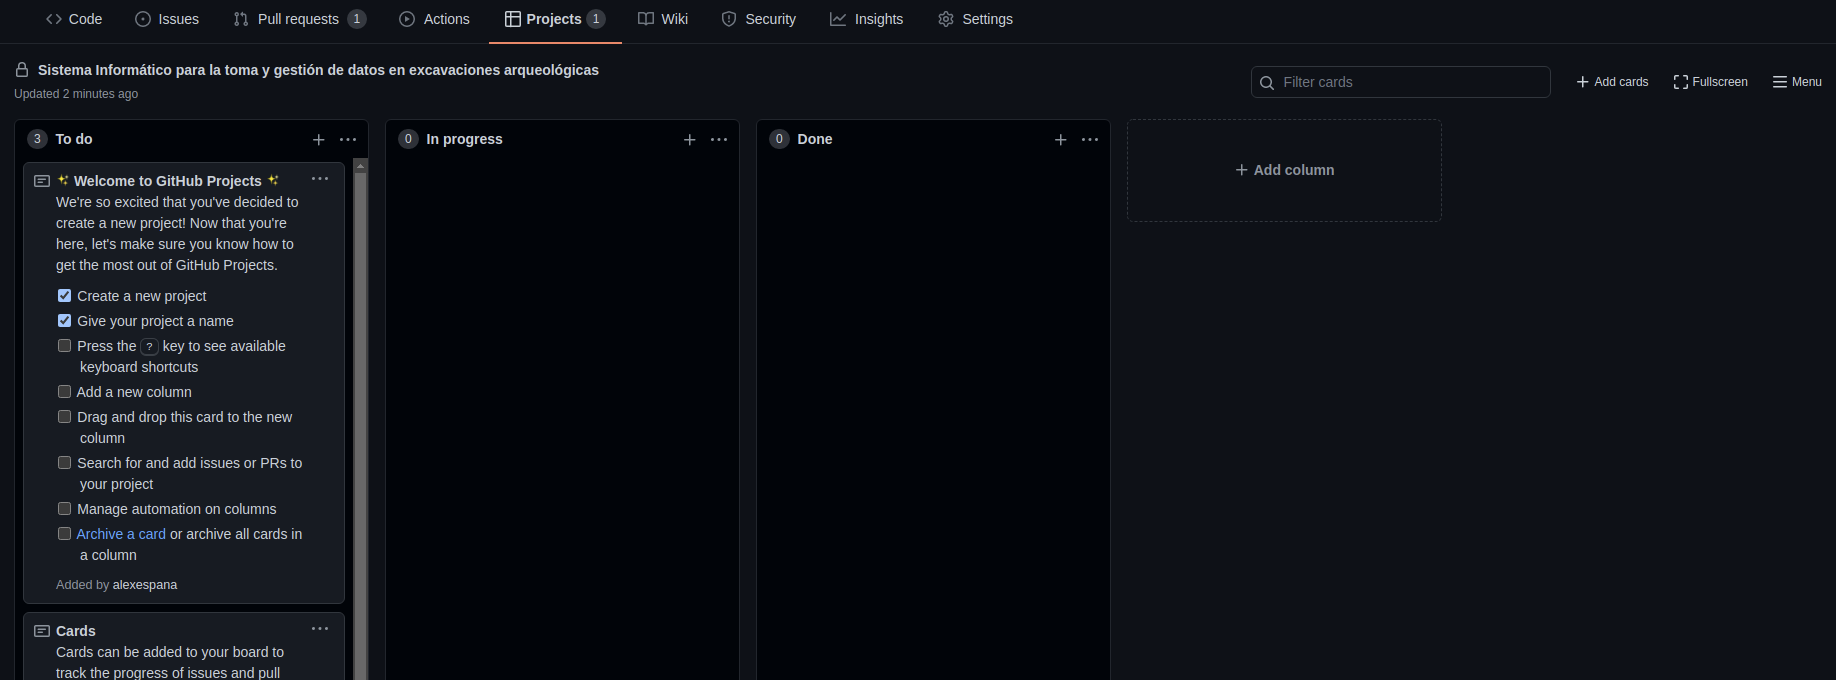
\includegraphics[scale=0.19]{imagenes/project-board.png}
        \caption[Tablero del proyecto]{Tablero del proyecto. Fuente \cite{project-board-image}}
        \label{fig:project-board}
    \end{figure}

    \begin{itemize}
        \item \textbf{To Do}: corresponde a los \textit{issues} en los que no se ha empezado
        a desarrollar.
        \item \textbf{In Progress}: corresponde a los \textit{issues} que se están
        desarrollando.
        \item \textbf{Done}: corresponde a los \textit{issues} que ya se han completado.
    \end{itemize}

Además, se han utilizado opciones de \textbf{automatización de los tableros}
\cite{automatic-project-board}, es decir, plantillas ya predefinidas que nos mueven las
\textit{issues} automáticamente de una columna a otra según determinados eventos, lo que
facilita en gran medida la organización del proyecto.\\

Pasando a hablar desde el punto de vista de las reuniones para el seguimiento del proyecto,
además de utilizar las herramientas mencionadas anteriormente, se han ido realizando diversas
reuniones presenciales o por videoconferencia con el tutor académico \textit{Daniel Sánchez
Fernández} para supervisar que el proyecto se estuviera desarrollando de forma correcta.
Dichas reuniones se han ido manteniendo conforme se han requerido, normalmente cada dos
semanas se ha realizado una pequeña reunión para supervisar el trabajo o para comentar dudas
o dificultades encontradas durante la implementación. Todas estas reuniones se han reflejado
en el Anexo \ref{ch:meetings} que puede encontrarse al final del documento.

	% Análisis del problema
	% 1. Análisis de requisitos
	% 2. Análisis de las soluciones
	% 3. Solucion propuesta
	% 4. Análisis de seguridad
	\chapter{Análisis del problema}
 
En todo proceso de Ingeniería del Software se necesita seguir un procedimiento muy metódico
y preciso, dividiendo el desarrollo del software en distintas fases que nos ayudarán a
conseguir un producto que se ajuste a las necesidades que requiere el problema.

\section{Ingeniería de requisitos}
Durante esta fase se cubrirán y proporcionarán las técnicas y los mecanismos apropiados
para:

    \begin{itemize}
        \item Analizar y entender las necesidades de los arqueólogos.
        \item Evaluar la viabilidad de las distintas propuestas (necesidades).
        \item Negociar un solución razonable/viable para ambas partes.
        \item Controlar y administrar los requisitos a lo largo del proceso de desarrollo.
    \end{itemize}

\subsection{Requisitos funcionales}
Describen la interacción entre la Aplicación Web y su entorno (base de datos, usuarios, 
comunicación con la App Android, etc), indicando cómo debe actuar
frente a situaciones o entradas determinadas.

    \begin{itemize}
        \item 
    \end{itemize}

\subsection{Requisitos no funcionales}
Este tipo de requisitos describen restricciones o cualidades de nuestra aplicación web que
no tienen una relación directa con las funcionalidades del sistema.

    \begin{itemize}
        \item 
    \end{itemize}

\subsection{Requisitos de información}
Este tipo de requisitos describirán necesidades de almacenamiento de información en
la aplicación web.

    \begin{itemize}
        \item 
    \end{itemize}

\section{Tecnologías disponibles}
En la elección de cualuquier herramienta en un proyecto software, se debe seguir un
proceso de selección de herramientas entre distintas alternativas, especificando claramente
los requisitos que deben cumplir para poder escoger aquella que mejor se adapte a las
necesidades del proyecto (en este caso a la aplicación web).

\subsection{Framework para desarrollo web}

    \subsubsection{Ruby on Rails}
    \textbf{Ruby on Rails} (también conocido como Rails) \cite{ruby-on-rails} es un framework
    para la creación de aplicaciones web escrito en Ruby. Sigue una arquitectura
    (Model-View-Controller) y diseño RESTfull. Está diseñado para facilitar la programación
    web al hacer una estimación de los componentes principales que se necesitan para comenzar.

    Este software asume que hay una mejor forma de hacer las cosas y está diseñado para
    ello, por lo que es un código muy optimizado y hecho para aumentar la productividad
    si se hace el desarrollo de la forma "The Rails Way".

    \subsubsection{Django}
    \textbf{Django} \cite{django} es el framework para Python más usado, está enfocado a sitios
    basados en bases de datos. Permite un desarrollo software muy rápido y limpio. Tiene una
    arquitectura MVT (Model-View-Template), donde el View sería el equivalente a Controller
    en MVC.

    Al igual que el anterior framework mencionado, Django ha sido diseñado por programadores
    experimentados, y se encarga de las partes más complejas del desarrollo web, permitiendo
    que el programador se centre en escribir la aplicación sin necesidad de preocuparse
    por otras cuestiones.

    \subsubsection{Laravel}
    \textbf{Laravel} \cite{laravel} es el mejor framework de PHP para desarrollar aplicaciones
    y servicios web con PHP5, PHP7 y PHP8. Al igual que Ruby on Rails, sigue una arquitectura 
    MVC, por lo que es sencillo relacionar las distintas componentes de la aplicación.

    Es un framework moderno que ofrece muchas utilidades a los desarrolladores y permiten un
    desarrollo ágil de las aplicaciones web. Además, pone mucho interés en la calidad del
    código, el mantenimiento y la escalabilidad.

    \subsubsection{Angular}
    \textbf{Angular} \cite{angular} es un framework desarrollado en TypeScript para el
    desarrollo de aplicaciones web. Está mantenido por Google, utilizado para crear y mantener
    aplicaciones SPA (Single Page Application), es decir páginas web que interaccionan con el
    usuario dinámicamente sobreescribiendo la página con información nueva.

    Al contrario que los frameworks anteriormente mencionados, Angular no usa un modelo MVC
    o MVT, sino que permite el desarrollo del front-end y el back-end de forma totalmente
    independiente.

\subsection{Framework CSS}

    \subsubsection{Tailwind CSS}
    \textbf{Tailwind CSS} \cite{tailwind-css} es un framework CSS que funciona escaneando los
    archivos HTML, componentes Javascript y otros templates generando los correspondientes
    estilos y escribiéndolos en un archivo CSS estático. No tiene muchos componentes, sino
    clases de utilidad que pueden aplicarse directamente sobre el código HTML del proyecto.
    Además de esto, permite una gran optimización del peso del código CSS mediante unos flujos
    de desarrollo.

        
    \subsubsection{Bootstrap}
    \textbf{Bootstrap} \cite{bootstrap} es uno de los frameworks más popullares y usados para
    el desarrollo de páginas web. Fue desarrollado por Twitter en 2010 para uso de la compañía
    pero más tarde pasó a ser código abierto. Este framework combina CSS y Javascript. Entre
    sus características fundamentales podemos encontrar:
    
    % \begin{list}{\textbullet}{ 
        %     \addtolength{\labelsep}{1mm}    % Distancia hasta la etiqueta
        %     \addtolength{\itemsep}{-2mm}    % Separación entre items
        %     \setlength{\itemindent}{5mm}}   % Identación de los items
        % \end{list}
        
        \begin{itemize}
            \item \textbf{Responsive design}: adaptación automática a distintos dispositivos
            como móviles y tablets.
            \item \textbf{Grid System}: posicionamiento de elementos en la página
            \item \textbf{Interface UI}: incluye formularios, botones, menús, etc.
        \end{itemize}
        
        \subsubsection{Foundation}
        \textbf{Foundation} \cite{foundation} es el principal competidor de Bootstrap, es un
        framework orientado Al desarrollo de sitios web totalmente responsives bajo el enfoque
        \textit{mobile first}, que es una metodología de desarrollo donde se tenga en cuenta
        en primer lugar los dispositivos móbiles. Esta metodología es totalmente contraria a
        la que usa Bootstrap ya que en él se usa   textit{Responsive Web Design} y en éste
        \textit{Mobile First Web Design}.
        
        Además de su metodología de desarrollo, posee ciertas características muy interesantes:
        
        \begin{itemize}
            \item \textbf{Fastclick}: eliminación del retraso al pulsar en dispositivos
            móviles.
            \item \textbf{Semántico}: todo es semántico, permitiendo tener un lenguaje de
            marcado limpio sin sacrificar su funcionalidad y velocidad.
            \item \textbf{Off Canvas}: creación de menús dinámicos
            \item \textbf{Customizable}: permite hacer diseño completamente personalizables,
            pudiendo eliminar elementos, definir el tamaño de las columnas, colores,
            fondos, etc
        \end{itemize}

    \subsubsection{Materialize CSS}
    \textbf{Materialize CSS} \cite{materialize-css} sigue el principio \textit{Material Design},
    es decir, ofrece componentes ya listos para ser utilizados, por supuesto responsive.
    Además, integra comportamientos dinámicos mediante JavaScript y no necesita de Jquery para
    funcionar.

    Entre sus principales caracterśiticas se encuentran:
        
        \begin{itemize}
            \item Al igual que otros frameworks mencionados, permite un diseño responsive.
            \item Permite crear menús laterales desplegables o abiertos según la resolución
            del dispositivo.
            \item Diseños utilizando la filosofía Material Design (colecciones, tarjetas,
            barras de navegación, modales, toast, etc).
            \item Añade utilidades como \textbf{Parallax} (técnica de diseño web en la que se crea
            un efecto de profundidad al hacer scroll)
        \end{itemize}

\subsection{Base de Datos}
Antes de pasar a la elección de la Base de Datos concreta necesitamos especificar si
necesitamos una base de datos SQL o una base de datos noSQL. 
\begin{itemize}
    \item \textbf{Bases de Datos SQL}: son aquellas que utilizan el lenguaje SQL (
    \textit{Structure Query Languaje}), un lenguaje de consulta estructurado. Este tipo de 
    bases de datos están formadas por filas y columnas. En cada una de las filas residen
    registros, mientras que las columnas corresponden a campos de los mismos. Son el tipo
    de bases de datos más estándarizado y con más uso actualmente.
    \item \textbf{Base de Datos noSQL}:  son aquellas bases de datos diseñadas para permitir
    grandes cantidades de datos (\textit{BIG DATA}), tipos de datos complejos, más índices,
    distintos tipos de consulta, etc. Este tipo de base de datos surgió para dar solución
    a los problemas de escalabilidad y rendimiento de las bases de datos relacionales en las
    que hay miles de usuarios concurrentemente y realizando millones de consultas.
\end{itemize}

En la siguiente tabla, se realiza una breve comparación entre ambos tipos: 

    \begin{table}[H]
        \begin{center}
            \begin{tabular}{ |l|l| } \hline
                \textbf{SQL} & \textbf{noSQL} \\ \hline
                Tablas & Hashes, listas \\
                Escalabilidad vertical & Escalabilidad horizontal \\
                Consistencia & Dinamicidad \\
                Datos estructurados & Big Data \\ \hline
            \end{tabular}
            \caption{tabla con la comparativa entre SQL y noSQL}
            \label{tab:databases}
        \end{center}
    \end{table}

Dada la naturaleza de nuestro problema, donde existe una clara jerarquización de los
elementos con los que se trabaja: \textbf{UE, sector, año, hecho, estructura}, ordenados
de menor a mayor complejidad, intuimos que necesitamos hacer uso de un sistema de
almacenamiento de información que cumpla con el esquema entidad-relación, por lo tanto,
deberemos usar una base de datos SQL. Las distintas bases de datos que podemos tantear
son las siguientes:

    \subsubsection{MySQL}
    \textbf{MySQL} \cite{mysql} más que una base de datos, es un sistema de gestión de bases
    de datos relacionales de código abierto (también conocido como RDBMS, Relational Database
    Management System). Es una de las bases de datos más populares en la actualidad y usa
    un modelo cliente-servidor.
    

    \subsubsection{SQLite}
    Al igual que mySQL, \textbf{SQLite} \cite{sqlite} es un RDBMS de tamaño reducido
    (aproximadamente 275 kiB) que a diferencia de otros RDBMS como mySQL que utilizan un
    modelo cliente-servidor, éste no es un proceso independiente con el que el programa
    principal se comunica, en este caso, se haría uso de llamadas a subrutinas y funciones
    integradas en el propio código fuente.

    \subsubsection{PostgreSQL}
    \textbf{PostgreSQL} \cite{postgresql} es un sistema de gestión de base de datos relacional
    que está orientado a objetos, de código abierto y además gratuito. Este RDBMS posee tipos
    de datos avanzados y permite optimizar de forma considerable el rendimiento, este tipo de
    características por lo general solo se ofrecen en sistemas de bases de datos privativas.
    Además de las características anteriormente mencionadas, permite un control de grandes
    volúmenes de datos y tiene soporte completo para \textbf{ACID} (\textit{Atomicity,
    Consistency, Isolation, Durability}).

\subsection{Solución propuesta}
Como se ha mencionado anteriormente, en cualquier elección de herramientas se debe señalar
claramente las características que debe cumplir para así poder descartar con facilidad
entre las disintas alternativas.

    \subsubsection{Elección del Framework de Desarrollo Web}
    El framework de Desarrollo Web debe cumplir con una serie de \textbf{requisitos} para
    su aceptación:

        \begin{enumerate}
            \item Que haga una deducción de los elementos principales de la aplicación,
            permitiendo centrarnos exclusivamente en el desarrollo de la misma.
            \item Que pueda permitir la configuración del mismo con distintas bases de
            datos.
            \item Que posea un sistema de gestión de usuarios (\textbf{autenticación}).
            \item Que el manejo de los modelos de la base de datos pueda abstraerse
            independientemente de la base de datos elegida mediante un \textbf{Object
            Relational Mapping} (ORM).
            \item Que incluya una fácil creación de la API para la posible comunicación
            con la App android.
        \end{enumerate}

    Tras tantear los distintos frameworks para el desarrollo de aplicaciones web disponibles
    se ha decidido utilizar Django, ya que está hecho en un lenguaje familiar para mí y
    además cumple todos los requisitos anteriormente mencionados.

    Dicho framework permite hacer lo siguiente:
        
        \begin{itemize}
            \item Crear la aplicación sin tener que preocuparnos de elementos para que
            ésta funcione.
            \item Configuración con distintas bases de datos, SQLite es la base de datos
            por defecto, pero además permite configurarlo para trabajar con mySQL y
            postgreSQL.
            \item Sistema de autenticación de usuarios, por lo que podremos gestionar el
            registro e inicio de sesión de los mismos.
            \item Contiene un ORM que permite el manejo de modelos de la base de datos
            abstrayendo la base de datos utilizada.
            \item A pesar de no venir incluido como tal, instalando la aplicación Django
            REST framework, es posible realizar la configuración de la API de una forma
            relativamente sencilla.
            \item Tiene una documentación realmente buena, clara y sencilla.
        \end{itemize}
    
    Éstas son las razones por las que se ha decidido elegir Django para el desarrollo de
    nuestra aplicación web.

    \subsubsection{Elección del Framework CSS}
    Entre los requisitos que el framework CSS debe cumplir están los siguientes:

        \begin{enumerate}
            \item Que permita un diseño responsive de la página web.
            \item Que siga la metodología Responsive Web Design.
            \item Que sea fácil de usar.
            \item Que esté actualmente mantenido por la comunidad.
            \item Que posea una documentación simple y fácil de entender. 
        \end{enumerate}

    Siguiendo los requisitos de arriba, Foundation puede ser descartado ya que no cumple el
    segundo requisito, ya que nuestra aplicación web principalmente va a estar diseñada para
    utilizarse en un ordenador (también podrá usarse en un smartphone, pero no es la
    finalidad).

    Entre los tres frameworks restantes, podría utilizarse cualquiera de ellos ya que cumplen
    con los requisitos, pero finalmente se ha decidido utilizar Bootstrap ya que es
    probablemente el framework más popular y sencillo de usar que hay, además de seguir
    siendo muy usado por la comunidad. 
    

    \subsubsection{Elección de la Base de Datos}
    Para la elección de la Base de Datos que utilizará el servidor web para almacenar toda
    la información de las excavaciones se tienen que cumplir los siguientes requisitos:

        \begin{enumerate}
            \item Que sea una base de datos relacional.
            \item Que sea open-source y gratuita.
            \item Que tenga soporte para la realización de transacciones seguras.
            \item Que haga un uso eficiente de los datos.
        \end{enumerate}

    Por cuestiones de escalabilidad, utilizar SQLite se puede descartar ya que posee un
    reducido número de tipos de datos y más bien está pensada para utilizarse en dispositivos
    con poca capacidad de almacenamiento.

    Ahora nos tocaría pensar en, ¿mySQL o postgreSQL? Realmente podría utilizarse cualquiera
    de las dos, pero posgreSQL ofrece algunas ventajas respecto a mySQL que merece la pena
    mencionar: 
    
        \begin{itemize}
            \item MySQL es propiedad de Oracle y podría pasar a ser un producto comercial
            (de pago), sin embargo, postgreSQL es \textbf{open source 100\%}.
            \item PostgreSQL ofrece una mayor \textbf{integridad y fiabilidad} de los datos
            (principio ACID).
            \item Gracias a funciones que lectura y escritura en paralelo, postgreSQL ofrece
            una mayor \textbf{velocidad} frente a mySQL.
        \end{itemize}
    
    Por estas razones, finalmente se ha decidido usar postgreSQL como base de datos para
    nuestro servidor web.


	% Desarrollo bajo sprints: 
	% 	1. Permitir registros y login de usuarios
	% 	2. Desarrollo del sistema de incidencias
	% 	3. Desarrollo del sistema de denuncias administrativas y accidentes
	% 	4. Desarrollo del sistema de croquis
	%   5. Instalación de la aplicación de manera automática
	\chapter{Implementación}

La implementación del software se ha dividido en hitos. Estos, han sido definidos en Github
y cada uno de ellos contiene un grupo de \textit{issues} que se corresponden con las distintas
mejoras que se han ido incorporando al software a lo largo de su desarrollo.\\



	% Presupuesto

	% Conclusiones
	\chapter{Conclusiones y trabajos futuros}



	% Trabajos futuros


	% Anexos del proyecto
	\renewcommand{\appendixname}{Anexo}
	\renewcommand{\appendixtocname}{Anexos}
	\renewcommand{\appendixpagename}{Anexos}

	\appendix
	\clearpage
	\addappheadtotoc
	\appendixpage
	
	% 1. Informe de tutorías
	\chapter{Informe de tutorías} \label{ch:meetings}
\section{1º Reunión (02/02/22): planteamiento general del TFG}
El proyecto consistirá en dos piezas fundamentales: una \textit{Aplicación Android} y un 
\textit{Servidor Web}. En este proyecto nos vamos a centrar en el Servidor Web, aunque en
fases posteriores será preciso hablar un poco de la aplicación Android para el establecimiento
de la comunicación entre la aplicación y el servidor, ya que será necesario un mutuo acuerdo
entre ambas partes.

    \subsection{Servidor Web}

        \begin{enumerate}
            \item Almacenamiento de información en el formato correspondiente.
            \item Introducción de información detallada (ficha completa).
            \item Posibilidad de edición de las imágenes tomadas (marcar dentro de las
            fotografías las zonas de interés).
            \item Posibilidad de crear un pdf con la información contenida en la base de
            datos.
        \end{enumerate}

    \subsection{Fichas para la recogida de información}
    Para la recogida de datos en arqueología se hace uso de una serie de fichas donde podemos
    distinguir dos:

        \begin{enumerate}
            \item Registro de campos: esta ficha está dividida en una ficha de datos,
            conteniendo información básica de la pieza estratigráfica y una ficha fotográfica,
            que contiene las imágenes que describen dicha unidad.
            \item Ficha completa: en dicha ficha se hace un informe más exhaustivo completando
            la ficha de registro de campos.
        \end{enumerate}

    \subsection{Aspectos a tener en cuenta}
    Para la realización de este proceso es necesario aplicar la Ingeniería del Software,
    realizando los \textit{diagramas de actividad} y \textit{diagramas relacionales} necesarios.
    Además sería interesante incluir un manual de uso para el usuario.

\section{2º Reunión (15/02/22): jerarquización de los elementos}
En esta segunda entrevista que tuvo lugar en la ETSIIT con el tutor Daniel Sánchez Fernández
y el arqueólogo Francisco Javier Brao Gonzalez se hablaron distintos temas, sobre todo de cara
al diseño de la base de datos, ya que pudimos deducir lo siguiente:

    \begin{enumerate}
        \item La aplicación web necesitaría una base de datos relacional.
        \item Las unidades estratigráficas no siempre están asociadas a un hecho, por lo
        que habría que tener en cuenta esto para el diseño de la base de datos.
        \item Cada excavación está identificada con un número, a partir de este número
        se asignan los sucesivos.
        \item Aunque las excavaciones se identifiquen con un número, nosotros trabajaremos
        con un identificador interno.
    \end{enumerate}

Además de esto, se habló de la toma de imágenes y del marcado de puntos en las mismas en el
registro de campos (\textit{Croquis Planta} y \textit{Croquis sección}). Para ello, la
aplicación Android tendría que enviar a la aplicación web los puntos de la imagen junto con
la imagen, luego, desde la aplicación web se tendrían que poder modificar dichos puntos mediante
alguna interfaz. 

Quedó pendiente por parte del arqueólogo la realización de un template de un posible informe
que se podría generar de una excavación. Para dicha generación, se cogerían los datos
que hay almacenados en la base de datos y se generaría un archivo word o un archivo similar,
que sea posteriormente modificable por el/la arqueólogo/a.


\section{3º Reunión (01/03/22): Diseño del modelo Entidad/Relación}
Una parte muy importante de la aplicación es la correcta modelización de la base de datos.
Para ello, \textit{Joaquín García Venegas} y yo hicimos un diseño inicial del modelo
E/R.

    \subsection{Entidades del modelo E/R}

        \begin{itemize}
            \item \textbf{Excavación}: es una entidad simple pero importante, ya que definirá
            la numeración (identificación) del resto de entidades del esquema 
            \item \textbf{Estancia}: compuesto por la asociación de hechos.
            \item \textbf{Hecho}: formado por un conjunto de unidades estratigráficas, que
            bien podrán ser tanto unidades estratigráficas sedimentarias como construidas 
            \item \textbf{Unidad estratigráfica}: es una de las entidades fundamentales de
            la base de datos, ya que es el nodo hoja en el árbol de la jerarquía.
            \item \textbf{Sedimentaria}: es una entidad que hereda de unidad estratigráfica.
            \item \textbf{Construida}: es una entidad que hereda de unidad estratigráfica.
            \item \textbf{Fotografía}: la poseen tanto las unidades estratigráficas como las
            estancias, serán las fotos descriptivas de una excavación
            \item \textbf{Inclusión}: entidad débil que surge como consecuencia de que una
            unidad estratigráfica de tipo sedimentaria puede contener restos de distintos
            componentes, haciendo necesaria la definición de una nueva entidad al modelo
            para poder reflejar una relación \textbf{muchos a uno entre Inclusión y
            Sedimentaria)}.
            \item \textbf{Material}: al igual que en la entidad anterior, surge con la
            necesidad de poder representar una relación \textbf{muchos a uno entre Material
            y Sedimentaria)}, ya que una unidad estratigráfica de tipo sedimentaria puede
            estar formada por muestras, metal, piedra, arcilla, etc.
        \end{itemize}


    \subsection{Dudas sobre el modelo} \label{subsec: doubts}
    Tras realizar el modelo, surgieron una serie de dudas acerca de las posibles relacionales
    y los datos de las fichas(tipos de datos y significado), lo cuál es normal ya que no
    dominamos los términos que se usan en arqueología con precisión. Las dudas que surgieron
    fueron las siguientes:

        \begin{enumerate}
            \item ¿Es el mismo material el de la ficha reducida que el de las unidades
            construidas?
            \item En la ficha de las estancias, no sabemos qué es el primer recuadro para
            dibujar.
            \item Problema de identificación de las estancias: en el pdf de metodologías, 
            se dice que se codifica con la palabra Estancia y tres dígitos (el primero
            indica la zona y los dos siguientes el nº de sector). Aparece un nº de sector,
            ¿es éste el nº de orden?
            \item ¿Son realmente importantes los atributos Plano nº, Seccion nº, Elevacion
            nº?
            \item ¿Una excavación puede pertenecer a varias UE?
            \item ¿El TPQ, TAQ y la fase en qué formato van, números, fechas, palabras, ..?
            \item ¿La ficha completa se rellena a partir de la ficha de campo?
            \item Las cotas, ¿van relacionadas con las pendientes?
        \end{enumerate}

    Evidentemente, estas dudas tendrán que ser resueltas por el arqueólogo Francisco Javier
    Brao Gonzalez en una reunión que se concertará posteriormente junto con el tutor,
    Daniel Sánchez Fernández.

\section{4º Reunión (07/03/22): Resolución de dudas}
En esta reunión se han resulto las dudas planteadas en la reunión anterior sobre el diseño
del modelo E/R. las correspondientes dudas junto a sus soluciones son las siguientes:

    \begin{enumerate}
        \item ¿Es el mismo material el de la ficha reducida que el de las unidades
        construidas? \textit{"No, el material de la ficha reducida corresponde a las
        unidades estratigráficas sedimentarias, mientras que el material de las
        construidas solo pertenece a éstas, además de ser único (es decir, una unidad
        construida no puede estar formada por distintos materiales)"}.
        \item En la ficha de las estancias, no sabemos qué es el primer recuadro para
        dibujar. \textit{"Este recuadro se corresponde con \textbf{la matriz de Harris}},
        dicha matriz se forma a partir de las UE en relación y los hechos en relación,
        colocando los distintos elementos correspondientemente en el recuadro".
        \item Problema de identificación de las estancias: en el pdf de metodologías, 
        se dice que se codifica con la palabra Estancia y tres dígitos (el primero
        indica la zona y los dos siguientes el nº de sector). Aparece un nº de sector,
        ¿es éste el nº de orden? \textit{"No, la zona y el sector siempre se rellenan,
        pero no forman parten de la identificación de la estancia. El nº de estancia
        no se forma a partir del númer de zona y el número de sector, un ejemplo podría
        ser por ejemplo con \textbf{ES001}, sin vinculación con el hecho"}.
        \item ¿Son realmente importantes los atributos Plano nº, Seccion nº, Elevacion
        nº? \textit{"Es simplemente documentación, son números que indican información
        de la Unidad Estratigráfica"}.
        \item ¿Una excavación puede pertenecer a varias UE? \textit{"No, normalmente una
        UE está asociada a una única excavación"}.
        \item ¿El TPQ, TAQ y la fase en qué formato van, números, fechas, palabras, ..?
        \textit{"El TPQ Y TAQ son números y la fase es un código ya definido que indica
        la época de la pieza (os tengo que pasar los códigos)"}.
        \item ¿La ficha completa se rellena a partir de la ficha de campo? \textit{"Sí,
        solo que hay que buscar la equivalencia entre algunos campos de la ficha
        reducida y la completa ya que cambian un poco"}.
        \item Las cotas, ¿van relacionadas con las pendientes? \textit{"Sí, la idea es
        que las zonas indiques la distancia que hay con respecto a un punto de referencia
        y luego las pendientes indican hacia donde está orientada la pieza: Norte-Sur,
        Suroeste-Este, etc, indican puntos de cardinalidad"}.
    \end{enumerate}

Tras esta reunión, se aclararon gran cantidad de dudas, lo que nos permitirá hacer un
correcto diseño del modelo E/R para su posterior paso a tablas y finalmente fusión, logrando
que el diseño de la base de datos sea correcto.

\section{5º Reunión (30/03/22): Corrección de memoria}
Tras el envío de la memoria de prácticas al tutor \textit{Daniel Sánchez Fernández}, se
han anotado una serie de recomendaciones a tener en cuenta en la memoria del proyecto. Entre
las anotaciones más relevantes destacan las siguientes:

    \begin{itemize}
        \item Es importante distinguir entre la elección de modelos en el diseño del problema
        y la elección de herramientas. Por ejemplo, elegir entre una base de datos relacional
        o noSQL sería una elección de diseño, mientras que elegir qué SGBD escoger (MySQL,
        SQLite, PostgreSQL, etc) sería una elección de herramientas.
        \item Incluir las citas desde las cuales se consulta la información.
        \item Comprobar que las imágenes usadas en la aplicación sean libres, o cambiarlas
        por imágenes de uso libre de repositorios como \href{https://pixabay.com/}{Pixabay} o
        \href{https://stock.adobe.com/es/}{Adobe Stock}.
        \item Dejar siempre claro la autoría de los archivos e imágenes incluidas en la memoria
        mediante una nota en la parte inferior de la misma o similar.
    \end{itemize}

Mencionadas estas anotaciones, se procede a modificar la estructura anterior de la memoria,
incluyendo un apartado nuevo dedicado al diseño. La sección de elección de herramientas
\ref{sec:tools} irá incluida en el capítulo de implementación, que recogerá la discusión de
herramientas elegidas y cómo se ha llevado a cabo la implementación de la aplicación.

\section{6º Reunión (16/05/22): prueba funcional de la aplicación}
Transcurridos más de dos meses desde el comienzo de la implementación del proyecto, se ha
vuelto a tener una reunión física con el tutor \textit{Daniel Sánchez Fernández} y el
arqueólogo \textit{Francisco Javier Brao Gonzalez}.\\

El principal objetivo de la misma es mostrar el funcionamiento de la aplicación al cliente, y
ver qué puntos le gustaría añadir o en qué puntos podría mejorar de cara a la entrega del
producto final. Tras esta reunión se propusieron los siguientes cambios al proyecto:

    \begin{enumerate}
        \item Es necesario mostrar el identificador de las unidades estratigráficas
        \textbf{precedido de las letras \textit{UE}}, para una mejor identificación de los
        elementos.
        \item Añadir un campo que sea el \textbf{nombre} de la excavación en las
        excavaciones.
        \item Añadir las \textbf{relaciones entre unidades estratigráficas}, es decir, en una
        unidad estratigráfica: la que está por encima y por debajo de la misma.
        \item Añadir si es posible un \textbf{sistema de log} en la aplicación para recoger
        todas las acciones realizadas por los usuarios. Estos logs podrán ser vistos por
        usuarios \textbf{staff} de la aplicación, es decir, arqueólogos con privilegios.
    \end{enumerate}

Estos cambios necesitarán ser añadidos a la entrega final del proyecto.


	% 2. Información sobre fichas y metodología
	\chapter{Documentación adicional}
\section{Fichas de registro} \label{sec:registrationforms}
En este documento se sitúan todos los campos necesarios para la recogida de datos de campo
y de registro completo. Así, en él se reflejan las \textbf{UE reducidas}, \textbf{UE
estratigráficas de registro completo},  \textbf{hechos}, \textbf{estancias}, el
\textbf{inventario fotográfico}, \textbf{mobiliario}, \textbf{cerámica} y \textbf{tipología},
aunque estos tres últimos no los abarcaremos ene este proyecto.

Este documento que se adjunta en primer lugar en la página siguiente \textbf{NO es de
autoría propia} y fue un documento proporcionado por el arqueólogo como apoyo documental.

\section{Metodología de registro}
En este documento, la parte principal y más importante describe \textbf{cómo se identifican
las entidades}, indicando el tipo de campos a los que se corresponden, enteros, palabras ya
previamente definidas como la letra identificativa de los Hechos junto con la numeración. Esta
información será de gran utilidad a la hora de elaborar el modelo E/R y tener claro qué
atributos forman la clave primaria y posibles claves candidatas de las entidades.

Este documento se adjunta en segundo lugar, después de \ref{sec:registrationforms}, e
igual que el anterior, \textbf{NO es de autoría propia} y fue un documento proporcionado por
el arqueólogo como apoyo documental.

% Fichas de recogida de datos, tanto de campo como completas
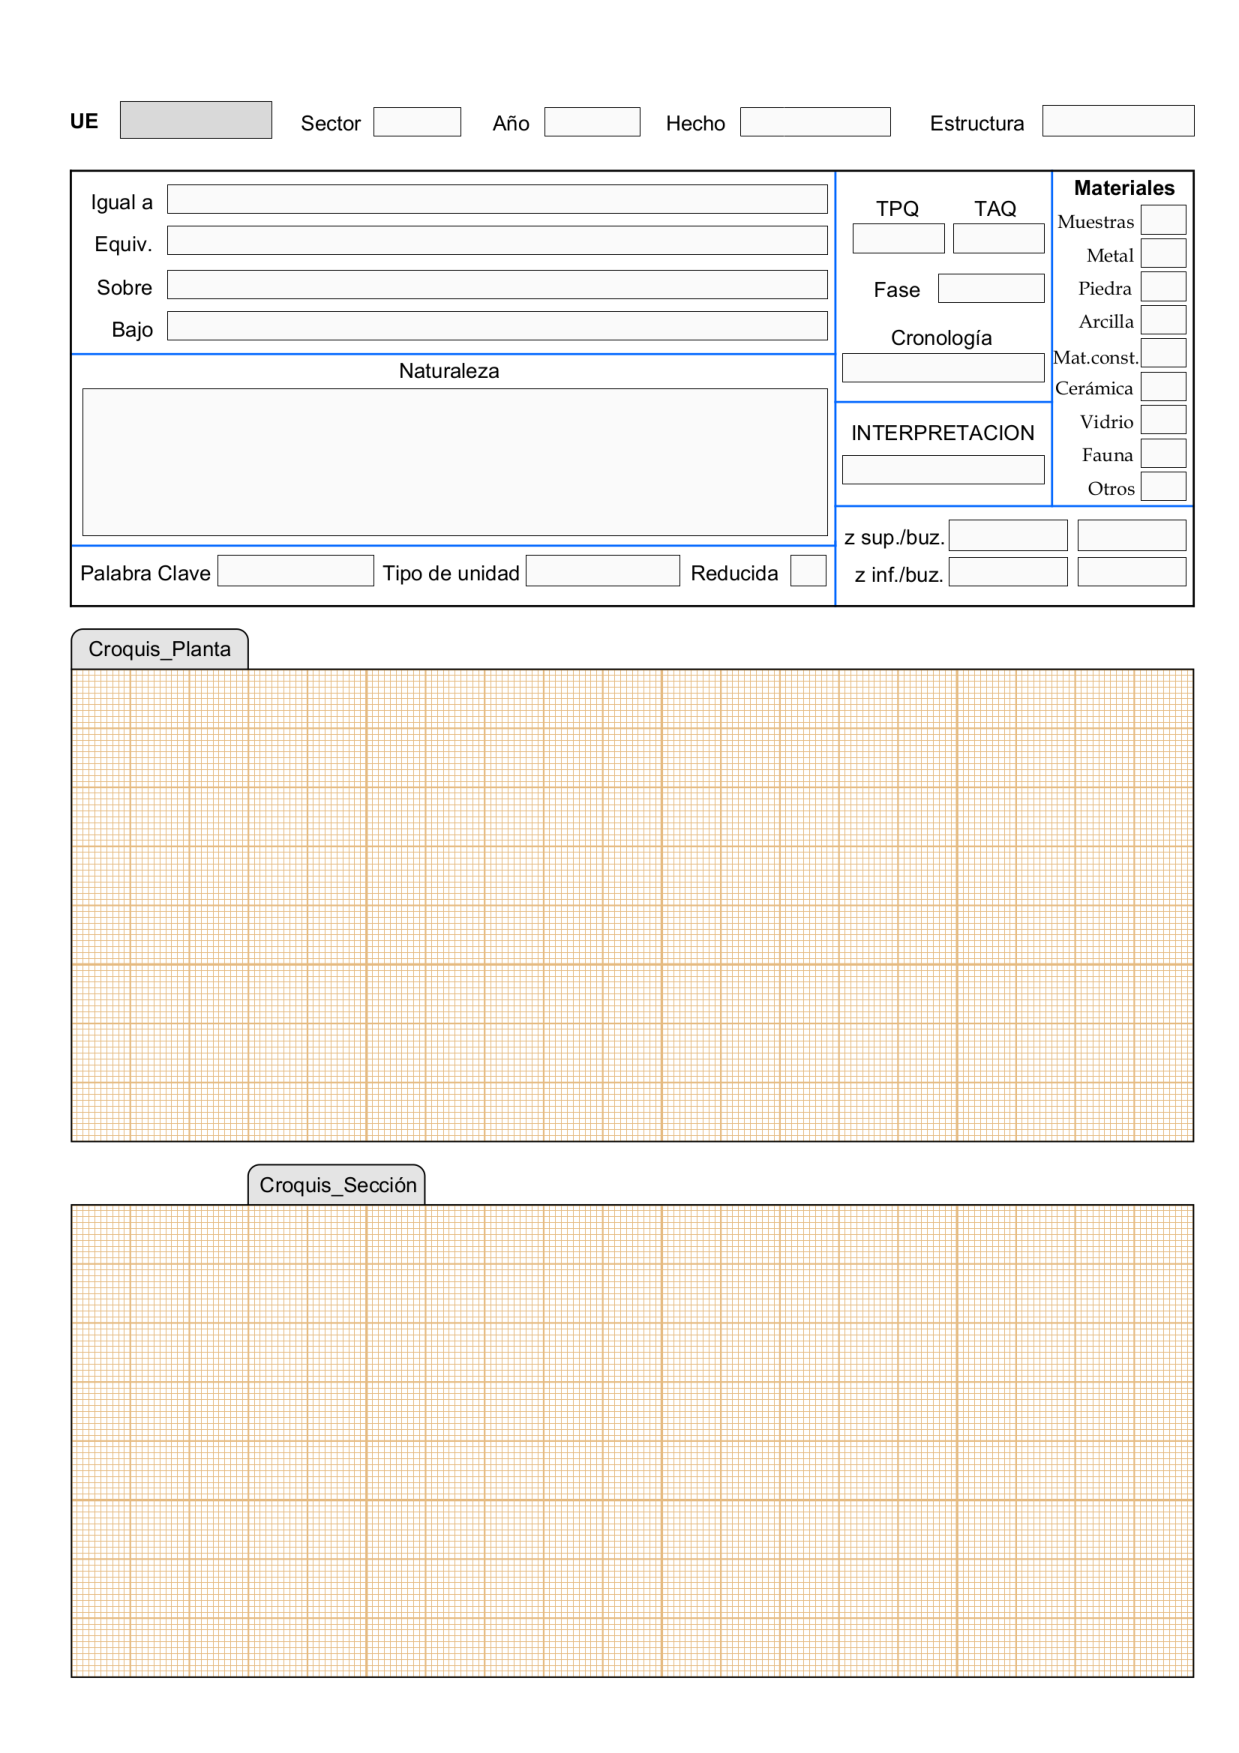
\includepdf[pages=1-7]{info/FichasRegistroCampoCompleto.pdf}

% Jerarquía entre los elementos e identificación de ellos
\includepdf[pages=2-3]{info/MetodologiaFichasRegistro.pdf}



	\newpage
	\bibliography{bibliografia}
	\bibliographystyle{plain}
	
\end{document}

